% =====================================================================
%  3.2 Exploratory data analysis (train years only)
% =====================================================================
\subsection{Exploratory Data Analysis}
\label{sec:eda}

The EDA uses only the training years 2015--2016, so that what we see cannot steer choices made on
validation.

\begin{figure}[H]
  \centering
  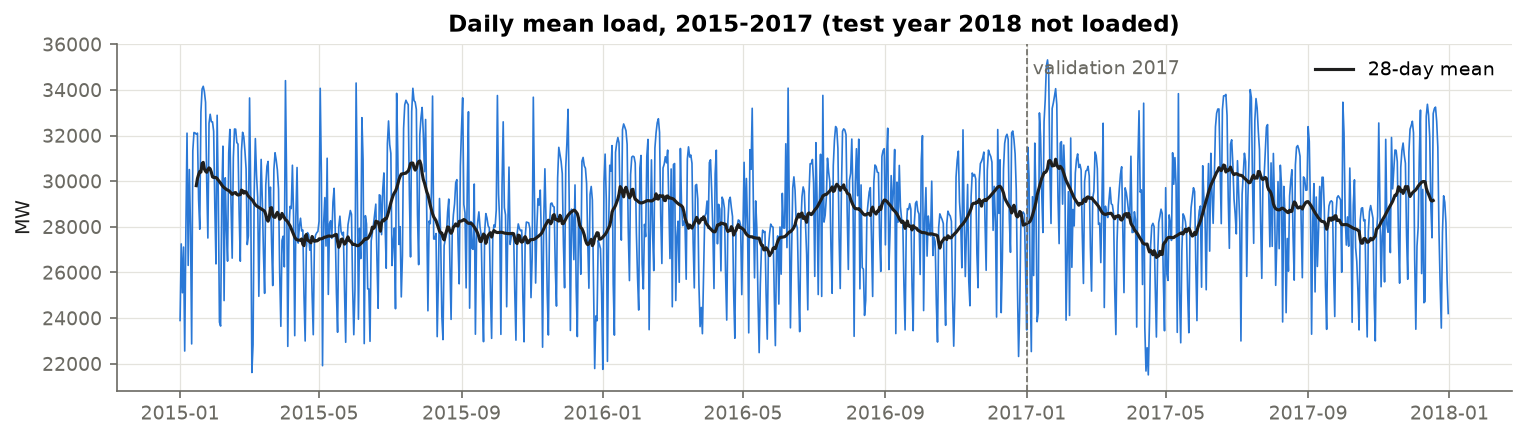
\includegraphics[width=\linewidth]{01_daily_load.png}
  \caption{Daily mean load with a 28-day moving average. The test year 2018 is not loaded.}
  \label{fig:daily-load}
\end{figure}

\Cref{fig:daily-load} shows a yearly cycle with winter and summer peaks, deep drops around
Christmas and in August, and a slow upward drift (annual means 28{,}391, 28{,}509 and 28{,}858\,MW
for 2015--2017).

\begin{figure}[H]
  \centering
  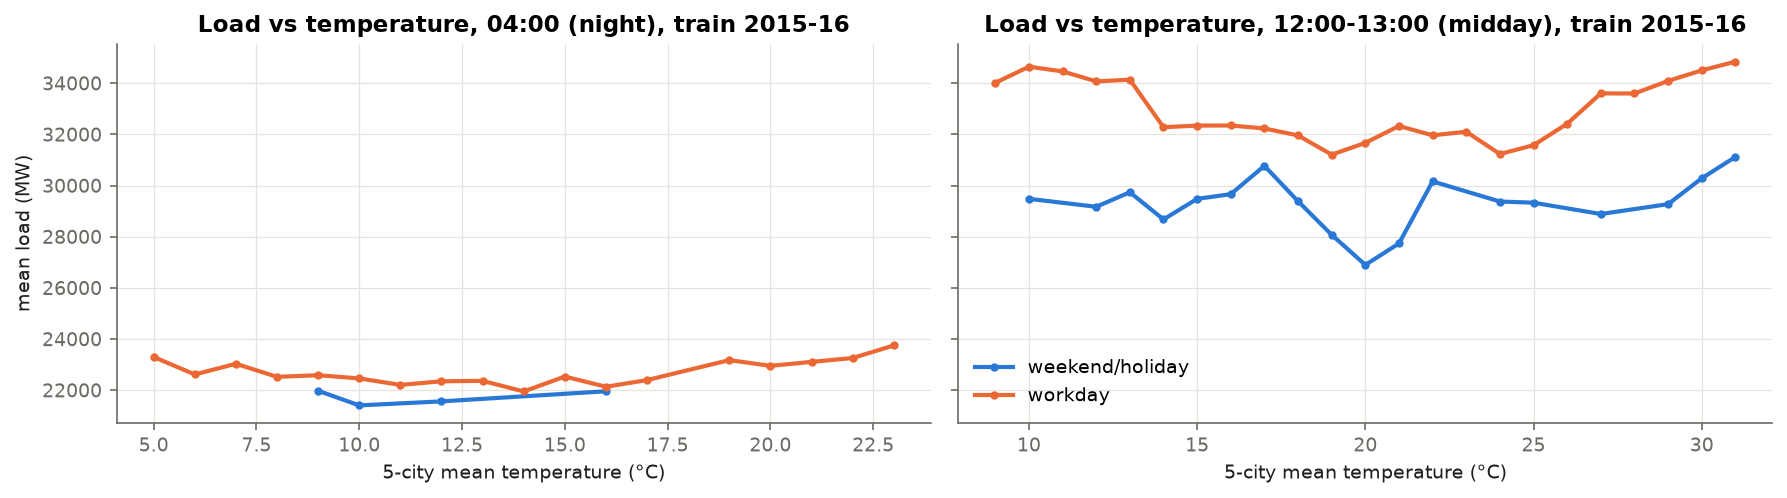
\includegraphics[width=\linewidth]{01_load_vs_temperature.png}
  \caption{Mean load per 1\,$^\circ$C temperature bin (bins with at least 15 hours), train years.}
  \label{fig:load-temp}
\end{figure}

At midday on workdays the U-shape is clear (\cref{fig:load-temp}): load is high below about
13\,$^\circ$C and above about 25\,$^\circ$C. At night the hot branch is weaker. However, cold
and hot days also differ in season, daylight and holidays, so this figure alone does not show that
temperature has its own effect.

\paragraph{Temperature effect within the same month.}
To remove the seasonal part we follow a rule fixed before looking at the data. Inside each cell of
hour $\times$ weekday $\times$ month $\times$ year (holidays and the Christmas window excluded), we
subtract the cell mean from both load and temperature and compute
$\beta=\sum \tilde y\,\tilde T/\sum \tilde T^2$. A branch passes if $\beta$ has the expected sign
(winter negative, summer positive) in \emph{both} years and its effect $|\beta|\,\mathrm{sd}(\tilde T)$
is at least 0.5\% of mean load. A second variant uses week instead of month cells.

\begin{table}[H]
  \centering
  \small
  \caption{Within-month temperature coefficient $\beta$ (MW/$^\circ$C) and effect of one standard
           deviation (\% of mean load), train years. A check mark means the year passes.}
  \label{tab:s2}
  \begin{tabular}{@{}l l rr rr@{}}
    \toprule
    & & \multicolumn{2}{c}{Month cells} & \multicolumn{2}{c}{Week cells} \\
    \cmidrule(lr){3-4}\cmidrule(l){5-6}
    Season & Year & $\beta$ & Effect & $\beta$ & Effect \\
    \midrule
    Winter (Dec--Feb) & 2015 & $+160$ & 1.24\% & $+76$ & 0.35\% \\
                      & 2016 & $-246$ & 1.88\% \checkmark & $-417$ & 1.59\% \checkmark \\
    July              & 2015 & $+79$ & 0.32\% & $+150$ & 0.55\% \checkmark \\
                      & 2016 & $+89$ & 0.59\% \checkmark & $-183$ & 0.96\% \\
    August            & 2015 & $-8$ & 0.04\% & $+154$ & 0.70\% \checkmark \\
                      & 2016 & $+440$ & 2.23\% \checkmark & $+572$ & 1.98\% \checkmark \\
    \bottomrule
  \end{tabular}
\end{table}

No branch passes in both years (\cref{tab:s2}). Winter 2015 has the wrong sign under both controls.
A possible reason is that most Spanish heating uses gas, so electric load reacts weakly to cold;
another is the quality of a five-city mean. Our data cannot separate the two. The summer effect is
mostly positive but small and unstable. We conclude that the U-shape in \cref{fig:load-temp} mostly
travels with the season. Temperature is still given to the models, but we do not claim a causal
``temperature drives load'' mechanism beyond seasonality.
